\chapter{LANDASAN TEORI}
% -------------------------------------------------------------------------------------------------------------------
% Konten:
% 1. Semantik web
% 2. Pemrosesan Bahasa Alami
% 3. Stemming ??? 
% 	a. algoritma stemming bahasa Indonesia ???
% 4. Ontologi
% 	a. Metode pembuatan ontologi
% 5. RDF
% 6. OWL Ontology
% 8. Ontologi Reasoning
% -------------------------------------------------------------------------------------------------------------------
Teknologi semantik web merupakan perluasan dari teknologi web yang telah ada saat ini atau lebih tepatnya adalah sebagai solusi dari kelemahan yang dimiliki oleh web saat ini. Seperti diketahui bahasa markup yang digunakan oleh web saat ini seperti HTML dan CSS hanya berfokus pada cara menampilkan dokumen saja tanpa memahami makna dari apa yang ditampilkannya. Akbiatnya, komputer tidak dapat memproses data lebih jauh lagi, seperti misalnya melakukan penyimpulan (inferensi) serta bertukar informasi antar website tanpa harus melibatkan peran pengguna.

\citet{liyang_yu} menyebutkan bahwa tujuan dari semantik web yaitu untuk mendapatkan informasi sebanyak mungkin mengenai sesuatu yang ingin kita gali, sesuatu di sini dapat berupa orang, acara, produk dan lain sebagainya hanya dengan melakukan query terhadap sekumupulan data yang sudah tersedia dalam website. Saat ini, kita tidak dapat mengetahui sebuah informasi yang terkandung dalam sebuah website hanya dengan melakukan query sederhana terhadap halaman web tersebut. Hal ini dikarenakan komputer tidak memahami infromasi yang ditampilkannya.

Penggunaan website saat ini sudah cukup beragam mulai dari membaca berita, berinteraksi dengan pengguna lain melalui media sosial maupun pencarian data dengan menggunakan mesin pencari seperti Google, Yahoo, Bing dan lain sebagainya. Melakukan pencarian data saat ini merupakan salah satu aktifitas yang paling banyak dilakukan oleh pengguna internet, namun dengan semakin banyaknya jumlah sumber data yang tersebar di internet mengakibatkan timbulnya permasalah baru yaitu susahnya mendapatkan informasi yang relevan dengan yang kita kehendaki, sebagai contoh misalnya kita ingin mencari infromasi mengenai program studi ilmu komputer Universitas Gadjah Mada dengan memasukkan kata kunci ``pascasarjana ilmu komputer UGM'' maka informasi yang akan kita dapatkan adalah tautan terhadap halaman-halaman yang mengandung kata-kata \emph{pascasarjana ilmu komputer ugm} yang jumlahnya dapat mencapai jutaan tautan. Hal ini tentunya akan menyebabkan proses untuk mendapatkan informasi yang sederhana seperti itu cukup memakan waktu karena selain kita harus membuka tautan yang diberikan mesin pencari tadi, kita juga harus membaca isi halaman tersebut untuk mengetahui apakah informasi yang disajikan sesuai dengan yang kita kehendaki atau tidak. Untuk itulah semantik web hadir memberikan jawaban atas persoalan ini.

\section{Bahasa} % (fold)
\label{sec:section_name}
Menurut \citet{chaer}, bahasa merupakan suatu lambang berupa bunyi, bersifat arbiter, digunakan oleh suatu masyarakat tutur untuk bekerja sama, berkomunikasi dan mengidentifikasi diri. \citet{dardjo}, bahasa adalah suatu lambang berupa bunyi, bersifat arbiter, digunakan oleh suatu masyarakat untuk bekerjasama, berkomunikasi,dan mengidentifikasi diri.
sebagai suatu sistem, bahasa memiliki aturan, kaidah atau pola-pola tertentu, baik dalam tata bunyi, tata bentuk kata, maupun tata kalimat. bahasa disusun oleh tiga komponen, yaitu: sintaksis, fonologi, dan semantik. Komponen sintaksis adalah komponen yang menangani ihwal yang berkaitan dengan kata, frasa dan kalimat. Komponen fonologi adalah komponen yang menangani ihwal yang berkaitan dengan bunyi. komponen semantik adalah komponen yang membahas ihwal makna \citep{dardjo}.

\subsection{Kata}
Menurut \citet{chaer} melalui \citet{admodjo} bahwa kata merupakan perwujudan bahasa sehingga bahasa tidak akan ada jika kata tidak ada. Setiap kata mengandung konsep makna dan mempunyai peranan dalam pelaksanaan bahasa. \citet{alwi} mengelompokkan kata ke dalam empat kategori sintaksis utama yaitu: verba, nomina, adjektiva dan adverbia.

\subsubsection{Verba (kata kerja)}
Kata-kata yang termasuk dalam kelompok kata kerja adalah kata-kata yang dapat diikuti oleh frasa \emph{dengan..} \citet{chaer}. Secara umum, verba berfungsi sebagai predikat atau inti predikat di dalam suatu kalimat \citep{alwi}. Dilihat dari perilaku semantisnya, verba memiliki makna inheren yang terkandung di dalam verba itu sendiri. Verba dapat mengandung makna inheren \emph{perbuatan (aksi), proses} atau \emph{keadaan yang bukan sifat atau kuantitas} \citep{alwi}.

\subsubsection{Adjektiva (kata sifat)}
Adjektiva adalah kata yang memberikan keterangan yang lebih khusus tentang sesuatu yang  dinyatakan oleh nomina dalam suatu kalimat \citep{alwi}. 

\subsubsection{Adverbia (kata keterangan)}
Adverbia adalah kata-kata yang digunakan untuk memberi penjelasan pada kalimat atau bagian kalimat lain, yang sifatnya tidak menerangkan keadaan atau sifat \citep{chaer}. Adverbia perlu dibedakan dalam tataran frasa dan dalam tataran klausa. Dalam tataran frasa, adverbia adalah kata yang menjelaskan verba, adjektiva dan adverbia lain. Sedangkan dalam tataran klausa, adverbia mewatasi atau menjelaskan fungsi-fungsi sintaksis \citep{alwi}.

\subsubsection{Nomina (kata beda)}
Kata benda adalah kata-kata yang dapat diikuti oleh frasa \emph{yang} ... atau \emph{yang sangat} ... \citep{chaer}. Dari segi bentuk morfologisnya, nomina dapat dibagi menjadi nomina dasar dan nomina turunan. Nomina dasar adalah nomina yang terdiri atas satu morfem sedangkan nomina turunan adalah nomina yang diturunkan melalui proses afiksasi, perulangan dan pemajmukan. Dari sisi semantisnya, kata benda mengacu pada manusia, binatang, benda dan konsep atau pengertian. \citet{alwi} mengungkapkan ciri-ciri nomina secara sintaksis adalah sebagai berikut:
\begin{enumerate}
	\item Dalam kalimat yang predikatnya berupa verba, nomina cenderung menduduki posisi sebagai subjek, objek atau pelengkap.
	
	\item Nomina tidak dapat diingkarkan dengan kata tidak.
	
	\item Nomina umumnya dapat diikuti dengan adjektiva, baik secara langsung maupun dengan diantarai oleh kata yang.
\end{enumerate}

\subsection{Frasa}
Frasa adalah gabungan dua buah kata atau lebih yang merupakan satu kesatuan. Tujuan dari penggabungan dua kata atau lebih menjadi satu kesatuan adalah untuk menampung konsep makna yang lebih khas atau lebih tertentu yang tidak dapat diwujudkan dengan sebuah kata saja \citep{chaer}. Secara sintaksis, frasa dapat dikelompokkan ke dalam frasa verbal, frasa nominal, frasa pronominal, frasa numeralia dan frasa preposisional. 

\subsection{Kalimat}
menurut \citet{alwi} melalui \citet{admodjo} kalimat adalah rentetan kata yang disusun sesuai kaidah yang berlaku. Tiap kata dalam kalimat mempunyai tiga klasifikasi, yaitu : kategori sintaksis, fungsi sintaksis, peran semantik. klasifikasi tersaji pada gambar 

\begin{figure}[ht]
	\centering
	\begin{lstlisting}[language=Prolog,xleftmargin=0pt]
	Kalimat            = Ibu     Memarahi   adi	

	Kategori Sintaksis = Nomina  Verba      Nomina 
	fungsi Sintaksis   = Subjek  Predikat   objek
	Peran semantik     = Pelaku  Perbuatan  Sasaran
	\end{lstlisting}
\caption{Klasifikasi Kata dalam sebuah kalimat}
\label{fig:klasifikasi_kata_dalam_kalimat}
\end{figure}

Menurut \citet{alwi}, kalimat merupakan konstruksi sintaksi terbesar yang terdiri dari dua kata atau lebih. Penggabungan dua kata atau lebih dalam satu kalimat menuntut adanya keserasian diantara unsur-unsur tersebut, baik dari segi makna maupun dari segi bentuk.

Kalimat dapat dikelompokkan berdasarkan jumlah kalusa yang menyusun kalimat. Klausa merupakan satuan sintaksis yang terdiri dari dua kata atau lebih yang mengandung unsur predikasi. Menurut \citet{alwi}, berdasarkan jumlah klausanya, kalimat dapat dibedakan menjadi:
\begin{enumerate}
	\item kalimat tunggal\\
	Kalimat tunggal adalah kalimat yang terdiri atas satu klausa. sehingga konstituen untuk unsur subjek dan predikat hanya ada satu atau merupakan datu kesatuan. Kalimat tunggal dapat mengandung unsur manasuka seperti keterangan tempat, waktu dan alat.

	\citet{alwi} melalui \citet{suryawan} membagi kalimat tunggal berdasarkan kategori predikatnya ke dalam kalimat  berpredikat verbal, kalimat berpredikat adjektival, kalimat berpredikat nominal (termasuk pronominal), kalimat berpredikat numeral dan kalimat berpredikat preposisional.

	\item Kalimat majemuk\\
	kalimat majemuk disusun oleh lebih dari satu klausa. Klausa-klausa yang terdapat di dalam kalimat majemuk bertingkat dapat dihubungkan dengan dua cara, yaitu: koordinasi dan subordinasi.

	Koordinasi adalah menghubungkan dua klausa atau lebih yang memiliki kedudukan konstituen sama. Kalimat majemuk yang dibentuk dengan menggunakan koordinasi disebut dengan \emph{kalimat majemuk setara}.

	Subordinasi adalah menguhubungkan dua klausa atau lebih yang kedudukan konstituennya tidak sama. Hubungan yang dibangun dengan menggunakan subordinasi dapat bersifat melengkapi (komplementatif) atau bersifat mewatasi atau menerangkan (atributif). Kalimat majemuk yang dibentuk dengan menggunakan subordinasi disebut dengan \emph{kalimat majemuk bertingkat}.
\end{enumerate}

Kalimat dapat dikelompokkan berdasarkan bentuk atau kategori sintaksis dari kalimat. Berdasarkan bentuk atau kategori sintakasisnya, kalimat dapat dibagi ke dalam empat kelompok, yaitu:
\begin{enumerate}
	\item Kalimat berita (kalimat deklaratif)\\
	Kalimat deklaratif umumnya digunakan untuk menyampaikan pernyataan sehingga isinya merupakan berita bagi pendengar atau pembacanya. Kalimat deklaratif tidak memiliki markah khusus, sehingga kalimat berita dapat berupa bentuk apa saja. Dalam bentuk tulisan, kalimat deklaratif diakhiri dengan tanda titik. Dalam bentuk lisan, kalimat berita diakhiri dengan nada turun.

	\item Kalimat perintah (kalimat imperatif)\\
	\citet{dardjo_et_al} mendefiniskan kalimat imperatif sebagai kalimat yang maknanya memberikan perintah untuk melakukan sesuatu. Dalam bentuk tulisan, kalimat imperatif diakhiri dengan menggunakan tanda seru (!). Dalam bentuk lisan, kalimat imperatif ditandai dengan nada yang semakin tinggi.

	\item Kalimat tanya (kalimat interogatif)\\
	\citet{dardjo_et_al} mendefinisikan kalimat interogatif sebagai kalimat yang isinya menanyakan sesuatu atau seseorang. Kalimat interogatif secara formal ditandai dengan kehadiran kata tanya seperti \emph{apa}, \emph{siapa}, \emph{berapa}, \emph{kapan} dan \emph{bagaimana}, dengan atau tanpa partikel penegas \emph{-kah}. Pada bahasa tulis, kalimat interogatif ditandai dengan tanda tanya (?). Pada bahasa lisan, kalimat tanya ditandai dengan suara naik jika kalimat memiliki kata tanya dan suara turun jika kalimat tidak memiliki kat tanya \citep{alwi}.

	Kalimat interogatif umumnya dibentuk dari kalimat deklaratif. Berikut adalah kaidah pembentukan kalimat tanya dari kalimat deklaratif menurut \citet{alwi}:

	\begin{enumerate}
		\item Kalimat tanya dapat dibentuk dari kalimat deklaratif dengan menambahkan pronomina penanya \emph{apa} pada kalimat tersebut. Partikel \emph{-kah} dapat ditambahkan pada pronomina penanya untuk mempertegas pertanyaan tersebut.

		\item Kalimat tanya dapat dibentuk dengan cara mengubah urutan kata dari kalimat deklaratif. Kaidah yang perlu diperhatikan dalam pembentukan kalimat tanya adalah sebagai berikut:
		\begin{enumerate}
			\item Jika dalam kalimat deklaratif terdapat kata seperti \emph{dapat, bisa, harus, sudah} dan \emph{mau}, maka kata tersebut dipindahkan ke awal kalimat dan ditambahkan partikel \emph{-kah}.

			\item Jika predikat dari kalimat berupa nomina atau adjektiva, urutan subjek dan predikatnya dapat dibalik kemudian partikel \emph{-kah} ditambahkan pada frasa yang telah dipindahkan ke awal kalimat.

			\item Jika predikat kalimat berupa verba taktrasitif, ekatransitif atau semitransitif, maka verba beserta objek atau pelengkapnya dapat dipindahkan ke awal kalimat dan kemudian ditambahkan partikel \emph{-kah}.
		\end{enumerate}

		\item Kalimat tanya dapat dibentuk dengan menempatkan kata \emph{bukan/bukankah, (apa/apakah) belum} atau \emph{tidak}.

		\item Kalimat tanya dapat dibentuk dengan mempertahankan urutan kata seperti dalam kalimat deklaratif, tetapi pengucapannya menggunakan intonasi yang naik.

		\item Kalimat tanya dapat dibentuk dengan menggunakan pronomina interogatif seperti \emph{apa, siapa, mengapa, kenapa, kapan, (Ke)berapa, dimana, kemana, dari mana, bagaimana} dan \emph{bilamana}.
	\end{enumerate}

	\item Kalimat seru (kalimat eksklamatif)\\
	Kalimat seru atau kalimat eksklamatif juga dikenal dengan sebutan kalimat interjeksi. Kalimat seru dapat digunakan untuk menyatakan perasaan kagum atau heran \citep{alwi}. \citet{chaer} menyatakan bahwa kalimat seru juga dapat digunakan untuk menyatakan emosi atau perasaan batin yang biasanya terjadi secara tiba-tiba.
\end{enumerate}

Kalimat dapat dikelompokkan berdasarkan kelengkapan unsur-unsur yang menyusun kalimat. Berdasakan kelengkapan unsurnya, kalimat dapat dikelompokkan ke dalam kalimat lengkap (kalimat major) dan kalimat tak lengkap (kalimat minor). Kalimat lengkap adalah kalimat yang memiliki unsur subjek dan predikat. Kalimat tak lengkap adalah kalimat yang tidak memiliki unsur subjek dan/ atau predikat. Kalimat tak lengkap umumnya muncul di dalam wacana dimana unsur yang tidak muncul tersebut sudah diketahui atau disebutkan sebelumnya \citep{alwi}.
% section section_name (end)
\section{\emph{Natural Language Processing} (NLP)} % (fold)

Penerapan Pengolahan Bahasa alami atau NLP pada sistem \emph{Information Retrival} (IR) dipercaya dapat dapat memperbaiki representasi tes dalam \emph{indexing} dan \emph{process searching} dibandingkan model yang sepenuhnya berbasis \emph{string matching}(Strzalkowski, dkk, 1999) melalui \citep{haryawan}.


% section tata_bahasa_indonesia (end)
\section{Gramatika}
Grammar suatu bahasa dapat dilihat sebagai suatu aturan yang menentukan apakah suatu kumpulan kata dapat diterima sebagai kalimat oleh bahasa tersebut. Sebuah bahasa L dapat dijelaskan sebagai satu kumpulan \emph{string}, dimana \emph{string} dibentuk dari bagian terkecil yang disebut dengan \emph{symbol}. Kelompok tertentu v dari \emph{symbol} biasa dikenal sebagai alfabet atau perbendaharaan kata. Sebuah kalimat yang dapat dikenali dibentuk dengan berdasarkan aturan-aturan tata bahasa yang biasa disebut \emph{grammar}.

Sebuah \emph{grammar} G dapat dibentuk dari empat buah \emph{tuple} yaitu: simbol non-terminal, simbol terminal, simbol awalan dan aturan penulisan atau \emph{rule} sehingga dapat ditulisakan sebagai $G=(vn, vt, s, p)$. Contoh pembentukan kalimat dengan mengacu pada \emph{grammar} G sederhana dapat dilihat dalam Gambar \ref{fig:pembentukan_grammar_g}.

\begin{figure}[ht]
	\centering
	\begin{lstlisting}[language=Prolog,xleftmargin=0pt]
		DictJenis = {Kata_Benda,Kata_Kerja,Frasa_Benda,Frasa_Kerja,Keterangan}
		DictKata = {Orang,Makan,Telur,Ayam,Terbang,Tinggi}
		
		dengan aturan:
	
		s           -> Frasa_Benda Frasa_Kerja
		Frasa_Benda -> Kata_Benda Kata_Benda
		Frasa_Kerja -> Kata_Kerja Keterangan
		Kata_Benda  -> {Orang,Telur,Ayam}
		Kata_Kerja  -> {Makan,Terbang}
		Keterangan  -> {Tinggi}
		
		Dari grammar G dapat dibentuk kalimat:
	
		Orang Makan Ayam
		Ayam Terbang Tinggi
		Orang Terbang Tinggi
		Ayam Makan Orang\end{lstlisting}
\caption{Contoh pembentukan kalimat dengan aturan gramatika}
\label{fig:pembentukan_grammar_g}
\end{figure}

Semua kalimat tersebut apabila dicari pembentukannya melalui \emph{grammar} G dapat dikatakan benar, akan tetapi harus diingat bahwa kalimat dengan \emph{grammar} yang benar hanya berarti benar secara struktural bukan berarti selalu benar dalam makna. Seperti kalimat ketiga yang hanya benar apabila berada dalam konteks `'orang memakai alat`' misalnya pesawat terbang. Sedangkan kalimat keempat malah sama sekali tidak mungkin dapat dimengerti maknanya, selain hanya akan menimbulkan tanda tanya bagi yang membaca. Dari \emph{grammar} kita dapat mempelajari bahasa dari segi struktur dan bukan dari segi makna bahasa itu sediri.

\citet{bar_feigenbaum} membagi \emph{grammar} ke dalam empat kelompok berdasarkan bentuk penulisan aturan produksi yaitu:
\begin{enumerate}
	\item \emph{Recursive enumerable grammar}\\
	\emph{Recursive enumerable grammar} atau tipe 0 merupakan tipe yang tidak membatasi jumlah simbol terminal dan non terminal untuk kedua sisi aturan produksinya. Kemampuan ekspresi \emph{(expressive power)} dari \emph{grammar} tipe ini sama dengan mesin turing.
	\item \emph{Contex-sensitive grammar}\\
	\emph{Context-sensitve grammar} atau \emph{grammar} tipe 1 memiliki ketentuan dimana simbol sisi kanan lebih banyak atau sama dengan simbol sisi kiri. \emph{Grammar} ini mampu merepresentasikan bahasa seperti $a\textsuperscript{n}b\textsuperscript{n}c\textsuperscript{n}$. Contoh \emph{grammar} tipe ini dapat dilihat dalam Gambar \ref{fig:contoh_csg}.
	\begin{figure}[ht]
		\centering
		\captionsetup{width=0.85\textwidth}
		\begin{lstlisting}[xleftmargin=30pt]
			S  -> aSBC
			S  -> aBC
			CB -> BC
			aB -> ab
			bB -> bb
			bC -> bc
			cC -> cc\end{lstlisting}
		\caption{Contoh \emph{Context-sensitive grammar} \citep{bar_feigenbaum}}
		\label{fig:contoh_csg}
	\end{figure}

	\item \emph{Contex-free grammar}\\
	Merupakan \emph{grammar} tipe 2 merupakan \emph{grammar} yang memiliki ciri yaitu sisi kiri hanya memiliki satu buah simbol non-terminal. Tiap-tiap aturan produksi dapat membuat simbol non-terminal dengan konteks yang bebas pada sisi sebelah kanan. \emph{Context-free grammar} populer digunakan untuk \emph{grammar} bahasa alami meskipun konstruksi beberapa bahasa alami tidak bersifat \emph{context-free}. Contoh \emph{grammar} tipe ini dapat dilihat dalam Gambar \ref{fig:contoh_cfg} berikut:
	\begin{figure}[hb]
		\centering
		\captionsetup{width=0.85\textwidth}
		\begin{lstlisting}[xleftmargin=30pt]
			<SENTENCE>    -> <NOUN PHRASE> <VERB PHRASE>
			<NOUN PHRASE> -> <DETERMINER> <NOUN>
			<NOUN PHRASE> -> <NOUN>
			<VERB PHRASE> -> <VERB><NOUN PHRASE>
			<DETERMINER>  -> the
			<NOUN> 		  -> boys
			<NOUN>		  -> apples
			<VERB>		  -> eat\end{lstlisting}
		\caption{Contoh penulisan aturan CFG untuk membentuk kalimat \citep{bar_feigenbaum}}
		\label{fig:contoh_cfg}
	\end{figure}


	\item \emph{Regular grammar}\\
	\emph{Regular grammar} atau tipe 3 adalah \emph{grammar} yang memiliki batasan yang paling ketat. Masing-masing aturan produksi memiliki sebuah simbol non-terminal pada sisi kiri. Masing-masing aturan produksi memiliki sebuah simbol terminal yang secara opsional dapat diikuti oleh sebuah simbol non-terminal pada sisi kanan.
\end{enumerate}
\section{\emph{Parsing}}
Menurut \citet{bar_feigenbaum} melalui \citet{suryawan}, \emph{parsing} adalah proses delinierisasi input linguistik, yaitu menggunakan sintak dan sumber pengetahuan lain untuk menentukan fungsi dari kata-kata yang terdapat di dalam kalimat untuk membentuk suatu struktur data seperti \emph{derivation tree} yang dapat digunakan untuk memperoleh makna kalimat. \citet{bar_feigenbaum} memandang \emph{parser} sebagai \emph{recursive pattern matcher} yang melakukan pencarian untuk memetakan string kata-kata ke dalam himpunan pola sintaksis yang bermakna.

Himpunan dari pola sintaksis yang digunakan oleh parser ditentukan oleh \emph{grammar} dari kalimat input. Secara teoritis, parser dapat memutuskan kalimat-kalimat yang termasuk dalam kalimat gramatikal dan dapat membangun struktur data yang merepresentasikan struktur sintaksis dari kalimat gramatikal yang ditemui dengan menggunakan \emph{grammar} yang kemprehensif \citep{bar_feigenbaum}.

Chomsky dan Postal dalam \citet{bar_feigenbaum} menyatakan bahwa secara umum bahasa alami tidak bersifat \emph{context-free}. Salah satu pendekatan yang digunakan untuk dapat mengakomodasi bahasa alami yang tidak bersifat \emph{context-free} adalah dengan menggunakan fitur di dalam \emph{grammar}.
\section{\emph{Resource Description Framework}}
\emph{Resource Description Framewok (RDF)} merupakan dasar pembentuk basis pengetahuan dalam semantik web, diajukan oleh W3C sebagai standar pada tahun 1999. RDF terdiri dari subjek, predikat dan objek yang kemudian dikenal dengan naman \emph{statement}. Subjek dapat berupa URI (Uniform Resource Identifier) yang berfungsi sebagai penanda atau \emph{identifier}, tidak menuntup kemungkinan sebuah subjek juga dapat berupa URL \emph{(Uniform Resource Locator)} yang merupakan bentuk khusus dari URI.  Predikat berupa URI yang menjelaskan hubungan antara subjek dengan objeknya sedangkan objek dapat berupa URI ataupun \emph{literal}. Sebuah pernyataan dalam RDF disebut dengan istilah \emph{triple}. secara grafis, bentuk \emph{statement} RDF dapat dilihat pada gambar \ref{fig:rdf_statement}.

\begin{figure}[ht]
	\centering
	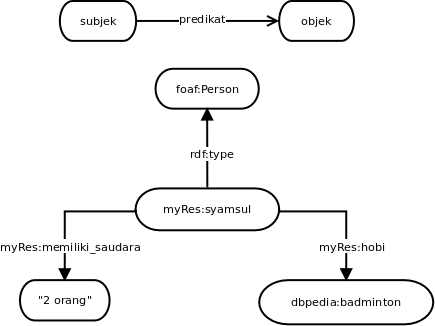
\includegraphics[trim = 29mm 141mm 40mm 0mm, clip, scale=0.6]{gambar}
	\caption{Struktur \emph{statement} RDF}
	\label{fig:rdf_statement}
\end{figure}

Sebagai contoh misalnya pernyataan ``Syamsul hobi badminton'', ``Syamsul memiliki saudara 2 orang'', pernyataan-pernyataan tersebut dapat dibentuk menjadi sebuah \emph{triple}. Pada pernyataan pertama, \emph{Syamsul} adalah merupakan subjek sedangkan \emph{hobi} merupakan sebuah predikat dan \emph{badminton} merupakan sebuah objek, sedangkan pada pernyataan kedua yang menjadi subjek adalah \emph{Syamsul} sedangkan predikat adalah \emph{memmiliki saudara} dan \emph{2 orang} merupakan objek. Jika objek pada pernyataan pertama di atas memerlukan penjelasan lebih lanjut, misalnya mengenai apa itu badminton, maka objek tersebut dapat berupa \emph{resource} dimana \emph{resource} tersebut membentuk triple-triple seperti terlihat pada gambar \ref{fig:rdf_multi_statement}. Pada pernyataan kedua, hanya dimungkinkan berupa literal karena tidak memerlukan penjelasan lebih lanjut mengenai objek itu sendiri.

Agar dapat di proses oleh komputer maka RDF triple harus dituliskan dalam bahasa atau sintak yang dapat dimengerti oleh komputer. Hingga saat ini bentuk penulisan RDF yang direkomendasikan oleh W3C adalah dalam bentuk XML dengan menggunakan namespace yang khusus RDF. Contoh statement di atas dapat kita serialisasi menjadi RDF sebagai berikut:
\lstinputlisting[firstline=1, lastline=7]{./parts/codeblock.xml}
\begin{figure}[ht]
	\centering
	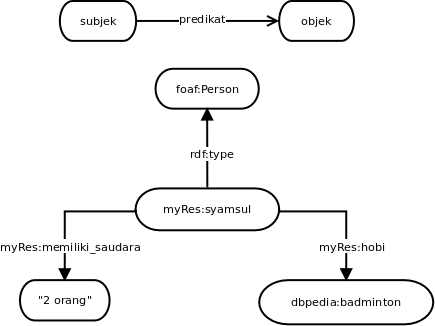
\includegraphics[trim = 0mm 0mm 0mm 93mm, clip, scale=0.55]{gambar}
	\caption{RDF dengan multi-statement}
	\label{fig:rdf_multi_statement}
\end{figure}
Selain XML/RDF, RDF juga dapat dituliskan dengan menggunakan Turtle sintaks sebagai berikut:
\lstinputlisting[firstline=9, lastline=11]{./parts/codeblock.xml}

Sintaks turtle lebih mudah dipahami oleh manusia, sehingga lebih mudah dibentuk. Meskipun sintak ini masih belum menjadi rekomendasi W3C namun besar kemungkinan kedepan juga akan menjadi rekomendasi karena sudah memiliki draft yang dapat dilihat di http://www.w3.org/TR/turtle/.
\section{\emph{RDF Schema}}
Dalam kasus yang lebih kompleks, RDF tidak cukup kuat untuk menjelaskan semantik dari sebuah subjek yang sedang dijelaskan. Jika kita kembali pada contoh di atas, apabila kita ingin lebih jauh menjelaskan mengenai misalnya apa/siapa Syamsul Muttaqin, RDF tidak dapat menjelaskan hal ini \citep*{antoniou}. Untuk mengatasi hal ini, maka di diperkenalkan RDF Schema (RDFS).

\begin{figure}[h]
	\centering
	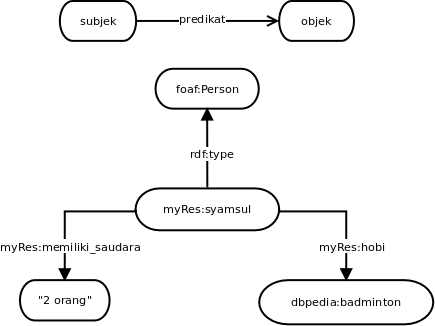
\includegraphics[trim = 0mm 0mm 0mm 32mm, clip, scale=0.55]{gambar}
	\caption{RDFS-statement}
	\label{fig:rdfs_statement}
\end{figure}

Sesuai dengan namanya, RDF Schema memberikan penjelasan lebih jauh mengenai objek yang sedang dibicarakan. Untuk itu RDFS diperkaya dengan beberapa penambahan namespace seperti rdfs:Class yang digunakan untuk menjelaskan tipe dari sebuah objek, rdfs:subClassOf yang merupakan turunan dari kelas, rdfs:domain, rdfs:range, serta beberapa penambahan lainnya. Gambar \ref{fig:rdfs_statement} menunjukkan RDFS statement, dimana \emph{foaf:Person} adalah kelas dan \emph{myRef:syamsul} merupakan \emph{instance} dari kelas \emph{Person}.
\section{Ontologi}
Ontologi memiliki peranan penting dalam semantik web. Terdapat berbagai definisi ontologi dalam bidanng semantik web, menurut T.R Gruber melalui \citet*{antoniou}, ontologi adalah \emph{spesifikasi formal dari sebuh konseptualisasi}, sedangkan W3C melalui \citet{liyang_yu} mendefinisikan ontologi sebagai \emph{definisi formal dari sekumpulan term yang digunakan untuk mendeskripsikan dan merepeserentasikan sebuah domain tertentu.}

Ontologi berfungsi sebagai media untuk berbagi pengetahuan dan pemahaman terhadap sesuatu antar domain atau berbagi terminologi yang berbeda namun memliki makna yang sama, misalnya \emph{ZIP Code} sama dengan Kode Wilayah di Indonesia, dengan demikian apabila seseorang mencari dengan menggunakan kata kunci kode wilayah untuk suatu daerah di Amerika misalnya, maka komputer akan dapat memahai bahwa yang dimaksud adalah ZIP Code, demikian juga sebaliknya.

\subsection{Metode pengembangan ontologi}
\citet{fernandez_lopez} melalui \citet*{fonou_huisman} menyebutkan berbagai macam metode yang dapat digunakan untuk pengembangan ontologi, namun demikian \citet{noy_mcguinness} mengungkapkan bahwa tidak ada satu metode yang pasti dalam mengembangkan ontologi. Ia juga mengungkapkan sesungguhnya proses pembuatan ontologi adalah sebuah proses iteratif yang tidak dapat dikerjakan hanya dalam satu tahapan saja, bahkan sangat mungkin pengembangan ontologi terus berlanjut meskipun ontologi sudah digunakan. 

Pemilihan metode pengembangan tergantung pada masing-masing pengembang ontologi, seperti misalnya \citet*{fonou_huisman} memilih menggunakan metode yang dikembangkan oleh \citet*{uschold_king} dengan alasan bahwa metode ini lebih mudah dipahami bagi para pengembang ontologi pemula.

\citet{noy_mcguinness} menawarkan salah satu metode pengembangan ontologi yang didasakan pada pengalaman mereka dalam mengembangkan ontologi. Metode ini paling banyak digunakan dalam pengembangan ontologi. Secara umum tahapan yang harus dilalui dalam pengembangan ontologi adalah sebagai berikut:
\begin{itemize}
	\item Tentukan domain dan ruang lingkup \emph{scope} dari ontologi\\
	Untuk membantu dalam menentukan domain dan ruang lingkup dari ontologi yang akan dibangun, seorang ahli ontologi \emph{ontology engineer} harus dapat menjawab pertanyaan:
	\begin{itemize}
		\item Domain apa yang ingin di-cover oleh ontologi ini ?
		\item Akan digunakan untuk apa ontologi ini ?
		\item Pertanyaan seperti apa yang harus dapat dijawab oleh ontologi ini ?
	\end{itemize}
	Jawaban atas pertanyaan-pertanyaan tersebut mungkin saja dapat berubah selama proses pengembangan ontologi berlangsung, namun setidaknya dapat membantu untuk memastikan ontologi yang akan dibangun tidak keluar dari rung lingkup yang sudah ditetapkan.
	\item Gunakan ontologi yang sudah ada\\
	Sebelum mulai mengembangkan ontologi, ada baiknya untuk mencari apakah ontologi yang akan dibuat sudah pernah dibuat atau belum. Jika sudah ada, apabila memenuhi kriteria yang diinginkan maka sebaiknya menggunakan ontologi tersebut.
	\item Tentukan semua \emph{term} penting dalam ontologi\\
	Tentukan semua \emph{term} baik berupa kelas, objek properti maupun \emph{datatype property} dari ontologi domain yang akan di-\em{cover}.
	\item Buat semua kelas dan strukturnya\\
	Pada tahapan ini, kelas-kelas yang akan di representasikan dalam domain dibuat terlebih dahulu, kemudian diikuti dengan membuat relasi antar kelas-kelas tersebut. Relasi disini termasuk struktur sub dan super kelas. Untuk menentukan struktur relasi dapat menggunakan metode \emph{top-down, bottom-up} atau kombinasi keduanya.
	\item Buat properti kelas - \emph{slot}\\
	Setelah proses pembuatan kelas selesai, selanjutnya buat juga properti yang akan digunakan pada kelas-kelas yang sudah dibuat.
	\item Tentukan \emph{facet} dari \emph{slot}\\
	\emph{Facet} menjelaskan mengenai tipe nilai dari kelas, nilai yang diperbolehkan, jumlah yang diperbolehkan \emph{(cardinality)}.
	\item Buat anggota dari kelas \emph{(instance)}\\
	Langkah terakhir adalah membuat anggota atau \emph{instance} dari masing-masing kelas.
\end{itemize}
\section{OWL Ontologi}
OWL \emph{(Web Ontology Language)} dijadikan sebagai rekomendasi formal oleh W3C pada 10 Februari 2004 \citep{liyang_yu}. OWL dirancang untuk kompatibel dengan sintak XML. OWL merupakan pengembangan RDF dan RDFS yang menjadi rekomendasi W3C sebelumnya, oleh karena itu secara sintaksis OWL kompatibel dengan sintak RDF dan RDF Schema.

Ide awal dari pengembangan OWL berdasarkan fakta bahwa RDF Schema belum cukup kuat dalam mereperesentasikan semantik dari sebuah \emph{statement} sehingga diperlukan definisi lebih lanjut. Definisi inilah yang kemudian diperkenalkan dalam OWL. \citet*{antoniou} menjelaskan beberapa model semantik yang tidak dapat dituangkan dalam RDF Schema diantaranya :
\begin{enumerate}
	\item Cakupan \emph{(scope)} dari sebuah properti. Sebagai contoh misalnya properti atau predikat \textit{memakan}, RDFS tidak dapat membatasi range cakupan properti ini hanya untuk kelas tertentu, misalnya kita tidak dapat menyebutkan ``Sapi hanya memakan rumput'', sementara sapi sendiri merupakan \emph{instance} dari kelas binatang, dimana kelas ini tidak hanya berisi sapi saja, namun juga dapat berisi kucing, sementara kucing tidak memakan rumput.
	\item \emph{Disjoint} antar kelas. RDFS hanya menjelaskan mengenai hirarki kelas--sub-kelas, ia tidak dapat membedakan apakah dua atau lebih kelas yang berbeda atau tidak. Sebagai contoh, misalnya kita ingin mendefinisikan kelas mobil dan motor adalah dua kelas yang berbeda, yang artinya apabila \emph{x} adalah \emph{instance} dari kelas motor, maka \emph{x} tidak mungkin menjadi \emph{instance} dari kelas mobil. RDFS tidak memiliki properti untuk menjelaskan hal ini, ia hanya dapat menjelaskan bahwa kedua kelas tersebut adalah merupakan sub-kelas dari kelas induk yaitu kendaraan.
	\item Kelas kompleks. RDFS tidak dapat mendefinisikan sebuah kelas baru yang merupakan gabungan (union) dari dua atau lebih kelas lain. RDFS juga tidak dapat mendefinisikan bentuk kombinasi lain seperti isrisan atau \emph{intersection} ataupun \emph{complement} dari dua buah kelas yang berbeda. Misalnya kelas Kendaraan adalah gabungan dari kelas Mobil dan Motor.
\end{enumerate}
Sebuah dokumen OWL terdiri dari elemen header, elemen kelas, elemen properti, elemen resktiksi properti, elemen properti khusus, serta elemen kombinasi boolean. 

\subsection{Elemen \emph{header}}
Sesuai dengan standar aturan XML dimana sebuah file terdiri dari sebuah elemen \emph{root}, elemen \emph{root} dari OWL adalah rdf:RDF dimana pada elemen \emph{root} ini dideklarasikan pula beberapa \emph{namspace} yang menjadi standar seperti terlihat pada Gambar \ref{fig:deklarasi_header_owl} berikut:
\begin{figure}[ht]
	\centering
	\lstinputlisting[firstline=13, lastline=16, xleftmargin=0pt]{./parts/codeblock.xml}
	\caption{Contoh deklarasi \emph{header} OWL}
	\label{fig:deklarasi_header_owl}
\end{figure}

Header terdapat diantara elemen \texttt{<owl:Ontology> </owl:Ontology>}. Header berisi informasi mengenai OWL yang bersagkutan seperti informasi versi, keterangan dan lain sebagainya. Contoh kode untuk mendefinisikan informasi mengenai OWL yang akan dibangun dapat dilihat dalam Gambar \ref{fig:deklarasi_informasi_owl} berikut:
\begin{figure}[hb]
	\centering
	\lstinputlisting[firstline=18, lastline=22, xleftmargin=0pt]{./parts/codeblock.xml}
	\caption{Contoh deklarasi informasi OWL}
	\label{fig:deklarasi_informasi_owl}
\end{figure}

\subsection{Elemen kelas}
Bagian selanjutnya adalah elemen kelas, bagian ini berada diantara elemen \texttt{<owl:Class></owl:Class>}. Sebuah kelas dapat terdiri dari beberapa sub kelas, seperti pada RDF Schema, apabila sebuah kelas merupakan sub dari kelas tertentu, maka definisinya dijelaskan di dalam elemen kelas tersebut. Gambar \ref{fig:deklarasi_kelas_owl} menunjukkan cara mendeklarasikan kelas dalam OWL.
\begin{figure}[hb]
	\centering
	\lstinputlisting[firstline=24, lastline=27, xleftmargin=0pt]{./parts/codeblock.xml}
	\caption{Contoh deklarasi kelas dalam OWL}
	\label{fig:deklarasi_kelas_owl}
\end{figure}

Elemen kelas pada Gambar \ref{fig:deklarasi_kelas_owl} mendefinisikan sebuah kelas bernama laki-laki yang memiliki hubungan \emph{disjoint} dengan kelas perempuan dan merupakan sub-kelas dari Person. OWL memiliki beberapa properti kelas selain \emph{disjoint} seperti equivalentClass yang digunakan untuk menjelaskan ekuivalensi sebuah kelas dengan kelas tertentu, disjointUnion untuk menjelaskan sebuah kelas dijoint dengan beberapa buah kelas yang digabungkan dan lain sebagainya.

\subsection{Elemen properti}
Elemen properti adalah elemen yang menjelaskan mengenai predikat dari sebuah statement, dimana predikat ini menjelaskan hubungan antar kelas atau antar \emph{instance} sebuah kelas dengan nilai dari properti \emph{instance} tersebut. Oleh karena itu elemen properti terdiri dari dua jenis yaitu object property dan datatype property.

\emph{Datatype property} menjelaskan hubungan antara \textit{instance} sebuah kelas dengan properti dari \textit{instance} tersebut, misalnya properti \textbf{umur} menjelaskan hubungan antara \textbf{person1} dengan sebuah literal value \textbf{"28"}. Gambar \ref{fig:deklarasi_dp_owl} menunjukkan cara melakukan definisi \emph{datatype property} dalam OWL.
\begin{figure}[hb]
	\centering
	\lstinputlisting[firstline=29, lastline=31, xleftmargin=0pt]{./parts/codeblock.xml}
	\caption{Contoh deklarasi \emph{datatype property} dalam OWL}
	\label{fig:deklarasi_dp_owl}
\end{figure}

\emph{Object property} menjelaskan hubungan antara sebuah kelas dengan kelas lainnya, misalnya properti diampuOleh menjelaskan hubungan antara kelas dosen dengan kelas matakuliah. Contoh deklarasi \emph{object property} diperlihatkan dalam Gambar \ref{fig:deklarasi_op_owl}.
\begin{figure}[ht]
	\centering
	\lstinputlisting[firstline=33, lastline=37, xleftmargin=0pt]{./parts/codeblock.xml}
	\caption{Contoh deklarasi \emph{object property} dalam OWL}
	\label{fig:deklarasi_op_owl}
\end{figure}

OWL juga memungkinkan kita untuk mendefinisikan inverse dari sebuah properti. Dari contoh di atas, elemen \texttt{<owl:inverseOf rdf:resource="\#mengampu" />} menjelaskan bahwa properti \textbf{diampuOleh} memiliki properti inverse yaitu mengampu, dimana nilai \texttt{rdfs:domain} dan \texttt{rdfs:range} dari properti mengampu merupakan kebalikan dari nilai \texttt{rdfs:domain} dan \texttt{rdfs:range} yang dimiliki oleh properti \textbf{diampuOleh}.

\subsection{Profil OWL}
Kemampuan OWL dalam membentuk ekspresi pengetahuan yang sangat lengkap memunculkan kendala dalam hal kemampuan komputer untuk melakukan \emph{reasoning}. Waktu komputasi yang dibutuhkan dalam proses reasoning dapat tidak terhingga, oleh karena itu kelompok kerja bidang ontologi di W3C seperti yang disebutkan oleh \citet*{mcguinness_vanharmelen} membagi OWL ontologi menjadi tiga buah sub bahasa berdasarkan batasan ekspresi logika yang dapat dibentuk yaitu:
\begin{enumerate}
	\item OWL-Full
	\item OWL-DL
	\item OWL-Lite
\end{enumerate}

\begin{figure}[ht]
	\centering
	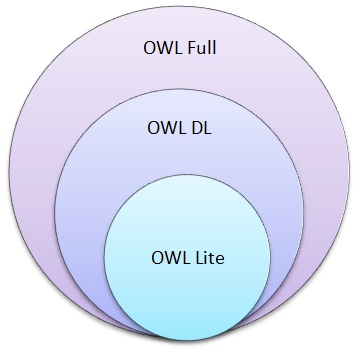
\includegraphics[width=0.3\textwidth]{bab_3/owl_subset.jpg}
	\caption{Diagram venn profil OWL 1}
	\label{fig:owl_subset}
\end{figure}

OWL-Lite merupakan sub-bagian dari OWL-DL, demikian juga dengan OWL-DL merupakan sub-bagian dari OWL-Full. Gambar \ref{fig:owl_subset} menunjukkan ilustrasi dari \emph{subset} OWL.


\section{OWL 2 Ontologi}
OWL terus dikembangkan seiring dengan semakin pesatnya perkembangan dan kebutuhan akan \emph{knowledge sharing}, oleh karena itu, kelompok kerja ontologi di W3C pada tahun 2012 menetapkan versi baru dari OWL yang disebut dengan OWL 2.0 atau OWL 2.

Bagian atas pada Gambar \ref{fig:owl_2_structure} menunjukkan format sintak yang dapat dipergunakan dalam menyusun ontologi dengan menggunakan bahasa OWL 2. Pada OWL 1, format yang dapat digunakan terbatas pada RDF/XML, sedangkan pada OWL 2 seperti yang terlihat dalam Gambar \ref{fig:owl_serialization_formats}. RDF/XML ditunjukkan pada baris 1 sampai 4, Functional Syntax ditunjukkan pada baris keenam, Manchester Syntax ditunjukkan pada baris ke 8 dan 9 sedangkan Turtle Syntax ditunjukkan pada baris ke sebelas. Dari semua format tersebut, W3C hanya mewajibkan format RDF/XML sebagai format standar, sedangkan format lainnya berupa opsional saja.

Masing-masing format sintak memiliki kelebihan dan kekurangan. Format RDF/XML memiliki dukungan yang paling baik, hanya saja kurang intuitif jika dibandingkan dengan Turtle, Functional maupun Manchester, sedangkan Turtle Functional dan Manchester tidak memiliki dukungan \emph{tool} yang baik \citep{liyang_yu}.

\begin{figure}[ht]
	\centering
	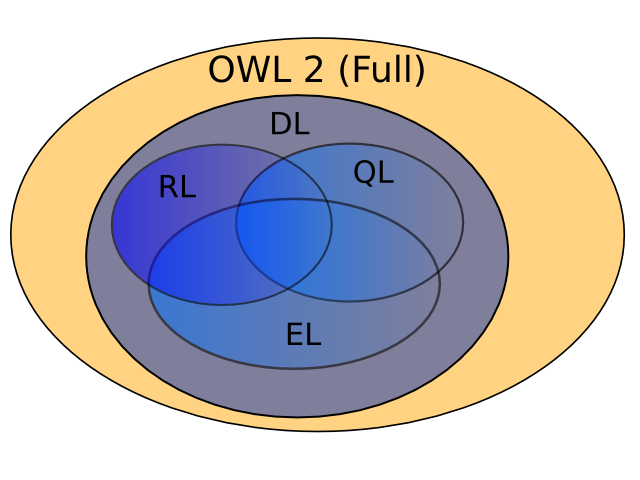
\includegraphics[width=0.3\textwidth]{bab_3/owl_2_profile}
	\caption{Diagram venn profil OWL 2}
	\label{fig:owl_2_profile}
\end{figure}

\begin{figure}[ht]
	\centering
	\begin{lstlisting}[language=XML, numbers=left]
	<SubClassOf>
		<Class IRI="Woman"/>
		<Class IRI="Person"/>
	</SubClassOf>

	SubClassOf( :Woman :Person )

	Class: Woman
		SubClassOf: Person

	:Woman rdfs:subClassOf :Person .\end{lstlisting}
	\caption{Contoh beragam format serialisasi OWL}
	\label{fig:owl_serialization_formats}
\end{figure}

\subsection{Profil OWL 2}
Seperti yang telah dijelaskan sebelumnya bahwa OWL 1 memiliki tiga sub-bahasa, namun dalam praktiknya ketiga sub-bahasa tersebut ternyata belum cukup untuk memenuhi kebutuhan yang ada. \citet{patel} mengungkapkan beberapa permasalahan dalam \emph{real world application} yang diadapi para pengembang. Untuk itu, OWL 2 terbagi ke dalam tiga buah profil, yaitu:
\begin{itemize}
	\item OWL 2 EL
	\item OWL 2 QL
	\item OWL 2 RL
\end{itemize}

Masing-masing profil dibatasi oleh batasan sintaks \emph{(syntactic restriction)}. Perlu diketahui bahwa sub-bahasa OWL 2 ini berdasarkan pada OWL-DL, sehingga semua ekspresi yang diyatakan valid pada OWL 2 EL misalnya, secara otomatis akan valid juga untuk OWL-DL. Gambar \ref{fig:owl_2_profile} menunjukkan diagram venn relasi antar sub-bahasa pada OWL 2.

\begin{figure}[ht]
	\centering
	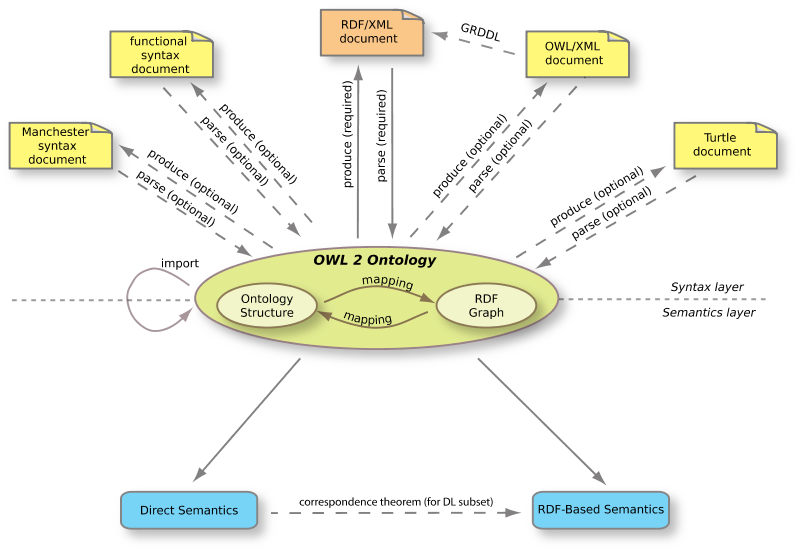
\includegraphics[width=0.8\textwidth]{bab_3/owl_2_structure}
	\caption{Struktur OWL 2.0}
	\label{fig:owl_2_structure}
\end{figure}
\section{Ontologi \emph{Reasoning}}
Proses \emph{reasoning} adalah proses untuk mendapatkan \emph{statement} yang terdapat dalam ontologi namun tidak dinyatakan secara implisit. \citet*{antoniou} menyebutkan beberapa hal yang dapat dihasilkan melalui proses \emph{reasoning} adalah:
\begin{itemize}
	\item Keanggotaan kelas \emph{(class membership)}. Menentukan apakah sebuah \emph{instance} merupakan anggota dari sebuah kelas. Penentuan keanggotaan ini dilakukan dengan cara memeriksa properti yang dimiliki oleh \emph{instance} tersebut.
	\item Klasifikasi. Apabila terdapat kelas bebek yang merupakan sub-kelas motor dan kelas motor sub-kelas dari kendaraan, maka dapat diperoleh \emph{statement} bahwa kelas bebek adalah sub-kelas dari kendaraan.
	\item Konsistensi dari sebuah ontologi. Untuk menentukan apakah sebuah ontologi konsisten seacara logika dapat pula dilakukan dengan menggunakan proses rasoning. Sebagai contoh, misalnya terdapat dua buah kelas mahasiswa dan dosen yang dinyatakan \emph{disjoint} dan terdapat satu buah \emph{instance} syamsul yang merupakan anggota dari kelas dosen dan mahasiswa, maka ontologi tersebut dikatakan tidak konsisten.
	\item Kesetaraan kelas \emph{equivalence of classes}. \emph{Reasoning} juga dapat digunakan untuk menentukan ekivalensi kelas, misalnya terdapat kelas kajur yang dinyatakan ekivalen dengan kelas karyawan dan kelas karyawan ekivalen dengan dosen, maka kelas kajur dengan dosen juga ekivalen. 
\end{itemize}
\section{SPARQL \emph{(Sparql Query Language)}}
SPARQL (diucapkan: ``sparkl'') adalah bahasa \emph{query} RDF \emph{(Resource Description Framework)} dan protokol untuk semantik web \citep{liyang_yu}. Secara harfiah, SPARQL adalah bahasa \emph{query} yang dapat kita gunakan untuk melakukan \emph{query} terhadap data dalam bentuk RDF dan SPARQL juga menyediakan protokol yang perlu kita ikuti jika ingin melakukan \emph{query} terhadap \emph{remote} RDF \citep{liyang_yu}. Tim Berners-Lee melalui \citet{ducharme} mengungkapkan ``Mencoba menggunakan semantik web tanpa SPARQL sama seperti menggunakan basis data relasional tanpa SQL''.

Rekomendasi W3C \emph{World Wide Web Consortium} mengenai SPARQL terdiri dari tiga bagian, yaitu:

\begin{enumerate}
	\item \emph{SPARQL query language specification} yang membahas mengenai inti dari bahasa \emph{query} SPARQL.
	\item \emph{SPAQRL Query XML Result Format specification} yang membahas mengenai format standar dari kembalian hasil \emph{query}.
	\item \emph{SPAQRL Protocol for RDF spesification} yang membahas mengenai protokol standar untuk mengakses RDF di lokasi yang berbeda \emph{(remote)}.
\end{enumerate}

Sparql terdiri dari empat buah bentuk \emph{query}, yaitu (1) SELECT, (2) ASK, (3) DESCRIBE dan (4) CONSTRUCT. Diantara keempat bentuk \emph{query} tersebut yang paling banyak digunakan adalah SELECT.

\subsection{\emph{SELECT Query}}
SELECT merupakan bentuk \emph{query} yang paling sering digunakan. Kebanyakan fiturnya juga digunakan pada bentuk \emph{query} lainnya (ASK, DESCRIBE dan CONSTRUCT). Bentuk dasar \emph{query SELECT} dapat dilihat pada Gambar \ref{fig:bentuk_query_select}.
\begin{figure}[hb]
	\centering
	\begin{lstlisting}[language=SQL, xleftmargin=15pt, numbers=left]
 	BASE <URI>
 	PREFIX pref: <URI>
 	...
 	SELECT <variabel1> <variabel2>
 	FROM <endpoint>
 	WHERE {
 		...
 	}\end{lstlisting} 
	\caption{Bentuk dasar \emph{query SELECT} \citep{liyang_yu}}
	\label{fig:bentuk_query_select}
\end{figure}

Query \emph{SELECT} diawali dengan mendefinisikan sebuah \emph{base} URI kemudian diikuti dengan \emph{PREFIX}. Jumlah \emph{PREFIX} tidak dibatasi sesuai dengan jumlah URI yang akan dilibatkan dalam melakukan \emph{query}. \emph{PREFIX} dapat pula tidak disertakan karena bersifat opsional. Jika tidak menggunakan \emph{PREFIX} maka \emph{URI} harus diuliskan dengan lengkap.

Klausa \emph{SELECT} digunakan untuk melakukan \emph{binding} terhadap data untuk menentukan data apa saja yang akan dikembalikan sebagai hasil \emph{query}. Klausa \emph{FROM} diletakkan setelah klausa \emph{SELECT}. Klausa ini berfungsi untuk menentukan alamat \emph{endpoint} yang akan dikenakan \emph{query}.

Bentuk \emph{query SELECT} sederhana ditunjukkan dalam Gambar \ref{fig:sparql_select_1}. Baris pertama mendeklarasikan \emph{base} URI, dimana \emph{base} URI merupakan alamat URI umum yang akan dijadikan acuan oleh semua URI yang dituliskan secara relatif di dalam \emph{query}. Pada Gambar \ref{fig:sparql_select_1}, URI relatif ditunjukkan dalam baris ke-6 dimana alamat URI lengkap dari <\#danbri> adalah <http://danbri.org/foaf.org\#danbri>. Perhatikan pada baris ke dua dalam Gambar \ref{fig:sparql_select_1} dapat dihilangkan karena bersifat opsional dan tidak pernah diacu dalam \emph{statement where}.

\begin{figure}[hb]
	\centering
	\begin{lstlisting}[language=SQL, numbers=left]
	base <http://danbri.org/foaf.rdf>
	PREFIX foaf: <http://xmlns.com/foaf/0.1/>

	select * from <http://danbri.org/foaf.rdf>
	where {
		<#danbri> ?propery ?value .
	}\end{lstlisting}
	\caption{Contoh klausa SELECT dalam \emph{query} SPARQL \citep{liyang_yu}}
	\label{fig:sparql_select_1}
\end{figure}

Contoh lain penggunaan klausa \emph{SELECT} dalam \emph{query} SPARQL dapat dilihat dalam Gambar \ref{fig:sparql_select_2}. \emph{Query} yang ditunjukkan dalam Gambar \ref{fig:sparql_select_2} terdiri dari tiga buah \emph{graph pattren} masing-masing ditunjukkan dalam baris 7, 8 dan 9. Berbeda dengan contoh sebelumnya, pada contoh ke dua ini \emph{PREFIX} tidak dapat dihilangkan karena digunakan dalam klausa \emph{where}. 

\begin{figure}[ht]
	\centering
	\begin{lstlisting}[language=SQL,numbers=left]
	base <http://danbri.org/foaf.rdf>
	PREFIX foaf: <http://xmlns.com/foaf/0.1/>
	PREFIX dc: <http://purl.org/dc/elements/1.1/>

	select * from <http://danbri.org/foaf.rdf>
	where {
		<#danbri> foaf:knows ?friend .
		?friend foaf:depiction ?picture .
		?picture dc:format ?imageFormat .
	}\end{lstlisting}
	\caption{Klausa \emph{SELECT} dengan banyak \emph{graph-pattern} \citep{liyang_yu}}
	\label{fig:sparql_select_2}
\end{figure}

\emph{Query} pada Gambar \ref{fig:sparql_select_2} akan menampilkan semua variabel yang terdapat di dalam klausa \emph{where}. Jika hanya ingin menampilkan variabel tertentu maka tanda ``*'' pada baris ke enam diganti dengan nama variabel yang ingin ditampilkan. Contoh \emph{query} seperti ini dapat dilihat pada Gambar \ref{fig:sparql_select_3}.

\begin{figure}[hb]
	\centering
	\begin{lstlisting}[language=SQL,numbers=left]
	base <http://danbri.org/foaf.rdf>
	PREFIX foaf: <http://xmlns.com/foaf/0.1/>
	PREFIX dc: <http://purl.org/dc/elements/1.1/>

	select ?friend,?image from <http://danbri.org/foaf.rdf>
	where {
		<#danbri> foaf:knows ?friend .
		?friend foaf:depiction ?picture .
		?picture dc:format ?imageFormat .
	}\end{lstlisting}
	\caption{Query untuk menampilkan nama dan foto}
	\label{fig:sparql_select_3}
\end{figure}

\subsection{\emph{Query} Terhadap Multi-Graph}
Contoh \emph{query} yang telah kita lihat pada sub bab sebelumnya hanya melibatkan \emph{graph} tunggal saja, namun demikian SPARQL memungkinkan kita untuk melakukan \emph{query} terhadap banyak \emph{graph} sekaligus dengan menggunakan metode \emph{named graph}.

Sebelum melakukan \emph{query} terhadap multi \emph{graph}, hal yang perlu diperhatikan adalah menyiapkan daftar \emph{named graph} yang akan kita \emph{query}. Definisi \emph{named graph} ditunjukkan dalam Gambar \ref{fig:definisi_named_graph}. Baris 2 dan 3 pada potongan \emph{query} dalam Gambar \ref{fig:definisi_named_graph} merupakan alamat URI graph yang akan dikenakan \emph{query}.

\begin{figure}[ht]
	\centering
	\begin{lstlisting}[language=SQL, numbers=left]
	select *
	from named <uri>
	from named <uri>
	...\end{lstlisting}
	\caption{Konstruksi \emph{query} terhadap multi \emph{named graph} \citep{liyang_yu}}
	\label{fig:definisi_named_graph}
\end{figure}
\section{SPARQL-DL}
\citet{evren_sirin} mengklasifikasikan bahasa query ontologi web semantik menjadi dua kelompok yaitu: bahasa query berbasis RDF \emph{(Resource Description Framework)} dan bahasa query berbasis DL \emph{(Description Logic)}. Bahasa query berbasis RDF ditujukan untuk melakukan query terhadap \emph{RDF Graph}. Bahasa query berbasis RDF diantaranya adalah SPARQL, SeRQL\footnote{http://rdf4j.org/} dan RDQL\footnote{http://www.w3.org/Submission/RDQL/}.

Ekspresi \emph{statement} bahasa query berbasis RDF seperti SPARQL, SeRQL dan RDQL berbasis pada bentuk \emph{RDF Triple} sehingga memiliki keterbatasan dalam melakukan query terhadap ontologi berbasis OWL 2 terutama OWL-DL. Misalnya terdapat ekspresi kelas dalam ontologi seperti ditunjukkan pada Persamaan \ref{eq:ekspresi_owldl} yang menyatakan bahwa terdapat sebuah kelas ``Dosen'' dengan kualifikasi anggota berupa individual dari kelas ``Orang'' yang memiliki relasi ``mengajar'' dengan individual kelas ``Mata\_Kuliah''. Apabila terdapat \emph{statement} seperti yang ditunjukkan pada Gambar \ref{fig:owl_entailment} maka SPARQL tidak dapat menemukan individual ``syamsul'' sebagai \emph{instance} kelas ``Dosen''.

\vspace{0.08cm}
\begin{equation}
	\label{eq:ekspresi_owldl}
	Dosen \equiv Orang \cap \exists mengajar.Mata\_kuliah 
\end{equation}
\vspace{0.08cm}

\begin{figure}[ht]
	\begin{lstlisting}[language=XML]
<ClassAssertion>
	<Class IRI="#Orang"/>
	<NamedIndividual IRI="#syamsul"/>
</ClassAssertion>
<ClassAssertion>
	<Class IRI="#Mata_Kuliah"/>
	<NamedIndividual IRI="#semantic_web"/>
</ClassAssertion>
<ObjectPropertyAssertion>
	<ObjectProperty IRI="#mengajar"/>
	<NamedIndividual IRI="#semantic_web"/>
	<NamedIndividual IRI="#syamsul"/>
</ObjectPropertyAssertion>\end{lstlisting}
\caption{Contoh ekspresi kelas ``Dosen'' dan Individual ``syamsul'' \emph{instance} dari kelas ``Orang''}
\label{fig:owl_entailment}
\end{figure}

Bahasa query berbasis \emph{Tripe pattern} tidak dapat mengekstraksi informasi berbasis ekspresi kompleks yang dihasilkan dari penggabungan definisi \emph{TBox} (class) dengan \emph{ABox} (individual). Beberapa penelitian yang dikemukakan untuk menangani keterbatasan bahasa query berbasis RDF diantaranya adalah \citet{evren_sirin}, \citet{kubias} dan \cite{fikes}. 

Bahasa query yang dikemukanan \cite{fikes} terbatas hanya pada query terhadap ekspresi \emph{TBox} sedangkan query SAIQL yang dikemukakan oleh \citet{kubias}. Bahasa query SPARQL-DL yang dikemukakan oleh \cite{evren_sirin} dapat diimplementasikan dengan menggunakan OWL-API. 

Arsitektur SPARQL-DL bekerja di atas \emph{library} OWL-API seperti ditunjukkan pada Gambar \ref{fig:sparqldl_architecture}. Bentuk \emph{statement} query SPARQL-DL mirip dengan \emph{statement} query SPARQL, perbedaan hanya terletak pada bentuk definisi klausa. Gambar \ref{fig:sparqldl_query_1} menunjukkan bentuk query SPARQL pada Gambar \ref{fig:sparql_select_1} jika ditransformasikan ke dalam bentuk SPARQL-DL. Contoh lain bentuk query SPARQL-DL ditunjukkan pada Gambar \ref{fig:sparqldl_query_2}. Ekspresi query yang didukung oleh SPARQL-DL cukup lengkap seperti ditunjukkan pada Tabel \ref{tab:sparqldl_expression}.

\begin{figure}[hb]
	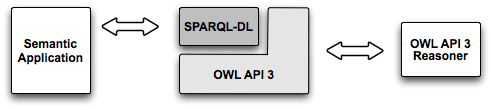
\includegraphics[width=1\textwidth]{bab_3/arsitektur_sparql_dl}
	\caption{Arsitektur SPARQL-DL}
	\label{fig:sparqldl_architecture}
\end{figure}

\begin{figure}[ht]
	\begin{lstlisting}[language=SQL, numbers=left]
PREFIX foaf: <http://xmlns.com/foaf/0.1/>
PREFIX : <http://danbri.org/foaf.rdf#>
select * where {
	PropertyValue(:danbri ?propery ?value)
}\end{lstlisting}
	\caption{Contoh query SPARQL-DL sederhana}
	\label{fig:sparqldl_query_1}
\end{figure}

\begin{figure}[ht]
	\begin{lstlisting}[language=SQL, numbers=left]
PREFIX wine: <http://w3.org/TR/2003/PR-owl-guide-20031209/wine#>
SELECT ?wine ?flavor WHERE { 
	PropertyValue(?wine, wine:locatedIn, wine:NewZealandRegion), 
	PropertyValue(?wine, wine:hasFlavor, ?flavor)
}\end{lstlisting}
	\caption{Contoh query SPARQL-DL dengan dua buah \emph{statement} kriteria}
	\label{fig:sparqldl_query_2}
\end{figure}

\begin{longtabu}{|c|l|X|}
	\caption{Daftar kelas ontologi geografi}\label{tab:sparqldl_expression}\\ \hline
	\textbf{No} & \textbf{Ekspresi Query}	&	\textbf{Keterangan}\\ \hline
	\endfirsthead
	\multicolumn{3}{c}%
	{\tablename\ \thetable\ {(lanjutan)}}\\ \hline
	\textbf{No} & \textbf{Ekspresi Query}	&	\textbf{Keterangan}\\ \hline
	\endhead
	1	&	Type(a,b)					&	\emph{a} adalah individual kelas \emph{b}\\ \hline
	2	&	Property(p)					&	\emph{p} adalah \emph{owl:Property}\\ \hline
	3	&	Class(a)					&	\emph{a} adalah \emph{owl:Class}\\ \hline
	4	&	Individual(a)				&	\emph{a} adalah \emph{owl:OWLNamedIndividual}\\	\hline
	5	&	PropertyValue(a, b, c)		&	\emph{a} memiliki properti \emph{b} dengan nilai \emph{c}\\ \hline
	6	&	EquivalentClass(a, b)		&	Kelas \emph{a} sama dengan \emph{b}\\ \hline
	7	&	SubClassOf(a, b)			&	\emph{a} sub kelas dari \emph{b}\\ \hline
	8	&	EquivalentProperty(a, b)	&	Properti \emph{a} sama dengan \emph{b}\\ \hline
	9	&	SubPropertyOf(a, b)			&	\emph{a} sub properti \emph{b}\\ \hline
	10	&	InverseOf(a, b)				&	Properti \emph{a} \emph{inverse} dari \emph{b}\\ \hline
	11	&	ObjectProperty(a)			&	\emph{a} adalah \emph{owl:ObjectProperty}\\ \hline
	12	&	DataProperty(a)				&	\emph{a} adalah \emph{owl:DataProperty}\\ \hline
	13	&	Functional(a)				&	\emph{a} memiliki karakteristik \emph{owl:Functional}\\ \hline
	14	&	InverseFunctional(a)		&	\emph{a} memiliki karakteristik \emph{owl:inverseFunctional}\\ \hline
	15	&	Transitive(a)				&	\emph{a} memiliki karakteristik \emph{owl:transitiveProperty}\\ \hline
	16	&	Symmetric(a)				&	\emph{a} memiliki karakteristik \emph{owl:symmetricProperty}\\ \hline
	17	&	Reflexive(a)				&	\emph{a} memiliki karakteristik \emph{owl:reflexive}\\ \hline
	18	&	Irreflexive(a)				&	\emph{a} memiliki karakteristik \emph{owl:irreflexive}\\ \hline
	19	&	SameAs(a, b)				&	\emph{a} memiliki karakteristik \emph{owl:sameAs}\\ \hline
	20	&	DisjointWith(a, b)			&	\emph{a} disjoint dengan \emph{b}\\ \hline
	21	&	DifferentFrom(a, b)			&	\emph{a} adalah individual yang berbeda dengan \emph{b}\\ \hline
	22	&	ComplementOf(a, b)			&	\emph{a} komplemen dari \emph{b}\\ \hline
	23	&	Annotation(a, b, c)			&	\emph{a} memiliki properti anotasi \emph{b} dengan nilai \emph{c} \emph{owl:Functional}\\ \hline
	24	&	StrictSubClassOf(a, b)		&	\emph{a} sub kelas (dengan aturan tertentu) dari \emph{b}\\ \hline
	25	&	DirectSubClassOf(a, b)		&	kelas \emph{a} berada langsung di bawah  \emph{b}\\ \hline
	26	&	DirectType(a, b)			&	individual \emph{a} merupakan \emph{instance} \emph{b} (sidpesifikan dalam \emph{statement})\\ \hline
	27	&	StrictSubPropertyOf(a, b)	&	\emph{a} sub properti (dengan aturan tertentu) dari \emph{b}\\ \hline
	28	&	DirectSubPropertyOf(a, b)	&	properti \emph{a} berada langsung di bawah  \emph{b}\\ \hline
\end{longtabu}
% \section{Ontology Merging}
%\input{./parts/BAB_3/question_answering}